\section{Independent evaluation against MODIS observations}
\label{sec:modis-evaluation}

The Fortran comparisons establish numerical consistency, but agreement with a
reference implementation does not establish physical realism. We therefore
evaluated the autonomous 2018 Torch integration against independent Terra
MODIS observations. Daily daytime and nighttime land surface temperature
(LST) came from the 0.05$^\circ$ MOD11C1 collection 6.1 product
\citep{Wan2021MOD11C1}. The collection-6 LST refinements are evaluated by
\citet{Wan2014MODISLST}. Fractional snow cover was taken from MOD10C1
collection 6.1 \citep{Hall2021MOD10C1}, whose data-record context is described
by \citet{Riggs2017MODISSnow}. Each of the 97,709 CMFD
land-column centres was assigned the containing MODIS CMG cell. This samples
the observations at the model locations but does not imply that the
satellite and model spatial supports are identical.

The evaluation integration starts from the common spun-up land state
described in Sect.~\ref{sec:fortran-torch-equivalence} (ERA5-Land 1~January~2005
state spun up for five years to the end of 2009 under CMFD forcing). This
spun-up restart is the initial state of every experiment in this section and
of the calibration, attribution, and closure experiments of
Appendix~\ref{app:modis-calibration} and Appendix~\ref{app:fortran-slab}.

MOD11C1 reports the UTC view time separately for each cell. The native
grid-mean radiative skin temperature of the model was sampled at the nearest
completed 1800~s physics step. The maximum timing displacement is therefore
15~min. The primary, strict LST mask requires successful production, zero
values in the mandatory and data-quality QC bits, and a stated LST error not
exceeding 1~K. A broader sensitivity mask retains produced retrievals with a
stated error not exceeding 2~K, includes many more retrievals under the
product's ``other quality'' category, and is reported separately.
MOD10C1 snow cover was compared with the prognostic SURF snow fraction at the
nominal Terra 10:30 local-solar-time overpass, requiring a spatial quality
flag of 0 or 1 and at least 50\,\% clear observations within the CMG cell.
All regional moments and categorical scores are weighted by
$\cos(\phi)$, and the observation operators are diagnostic and do not feed
back into the integration.

\begin{table}[H]
\caption{Area-weighted 2018 SURF evaluation against MODIS from the spun-up
initial state. Bias is SURF minus MODIS. The July--December snow row gives
the corresponding warm-season subset of the full-year snow statistics.}
\label{tab:modis-validation}
\centering
\small
\begin{tabular}{llrrrr}
\hline
Quantity & mask or period & samples & model mean & observed mean & bias / RMSE / $r$ \\
\hline
Daytime LST (K) & strict & 3,727,377 & 294.87 & 301.22 & $-6.37$ / 9.42 / 0.817 \\
Nighttime LST (K) & strict & 1,238,893 & 287.48 & 286.86 & 0.66 / 3.93 / 0.887 \\
Daytime LST (K) & broader QC & 19,857,571 & 286.51 & 289.89 & $-3.43$ / 7.72 / 0.899 \\
Nighttime LST (K) & broader QC & 20,904,460 & 274.02 & 272.16 & 1.79 / 5.53 / 0.933 \\
Snow fraction (-) & full year & 16,997,616 & 0.0492 & 0.0764 & $-0.0217$ / 0.192 / 0.575 \\
Snow fraction (-) & July--December & 8,642,926 & 0.0444 & 0.0624 & $-0.0177$ / 0.173 / 0.566 \\
\hline
\end{tabular}
\end{table}

The strict-QC results in Table~\ref{tab:modis-validation} distinguish the
daytime and nighttime behaviour. Nighttime LST has a small annual mean bias
of 0.66~K, an RMSE of 3.93~K, and a spatial-temporal correlation of 0.887.
Daytime LST instead has a $-6.37$~K bias and a 9.42~K RMSE. The broader QC
sample gives the same sign and seasonal structure but a smaller daytime bias
of $-3.43$~K; the strict clear-sky sample is not a random subset of the land
and atmosphere states, so both masks are shown rather than treated as an
uncertainty range.

The error is localized by the surface--air contrast. Under the strict mask,
the mean daytime surface-minus-air contrast is 4.88~K in SURF and 11.25~K in
MODIS; at night the corresponding values are $-2.95$ and $-3.61$~K. Over
snow-free columns ($3.04\times10^{6}$ strict samples) the daytime bias grows
monotonically with the observed contrast, from $+4.5$~K in the lowest decile
to $-17.7$~K in the highest, and regionally from $+0.7$~K over the humid
southeast to $-8.3$~K over the arid northwest and $-8.0$~K over the Tibetan
Plateau. The modelled day--night skin-temperature range at the view times
is 13.7~K against an observed 21.4~K. Where MODIS retrieves under the strict
mask the CMFD forcing is itself predominantly clear (view-time
transmissivity above 0.54 for 90\,\% of samples), so cloud-sampling
inconsistency affects a small minority. The daytime cold bias is therefore a
structural under-amplification of the daytime surface--air decoupling under
strong insolation, concentrated where the observed contrast is largest; it is
not a uniform offset, a masking artefact, or a night-time coupling error.
It is also shared by the Fortran reference rather than introduced by the
translation: the two implementations' 3-hourly grid-mean skin-temperature
archives agree over all 2{,}920 records of the year to a median absolute
difference of $1.0\times10^{-5}$~K and a 99th percentile of
$4\times10^{-3}$~K.

The model reproduces the broad seasonal retreat and re-establishment of snow
cover but underestimates the observed area-weighted snow fraction: for the
full year, fractional RMSE is 0.192 and correlation 0.575; at a 0.5
snow-cover threshold, the area-weighted probability of detection, false-alarm
ratio, and critical success index are 0.316, 0.381, and 0.265.
Figure~\ref{fig:modis-seasonal} condenses the annual behaviour into monthly,
area-weighted curves: the forecast follows the observed night-pass cycle
closely, under-amplifies the warm-season day-pass maximum, and tracks the
winter build-up and spring retreat of snow cover at a lower fraction than
observed. Snow-cover
extent is thus a further target for the observation-constrained experiments
below; it is not evidence that the numerical translation itself is
inaccurate.

\begin{figure}[t]
\centering
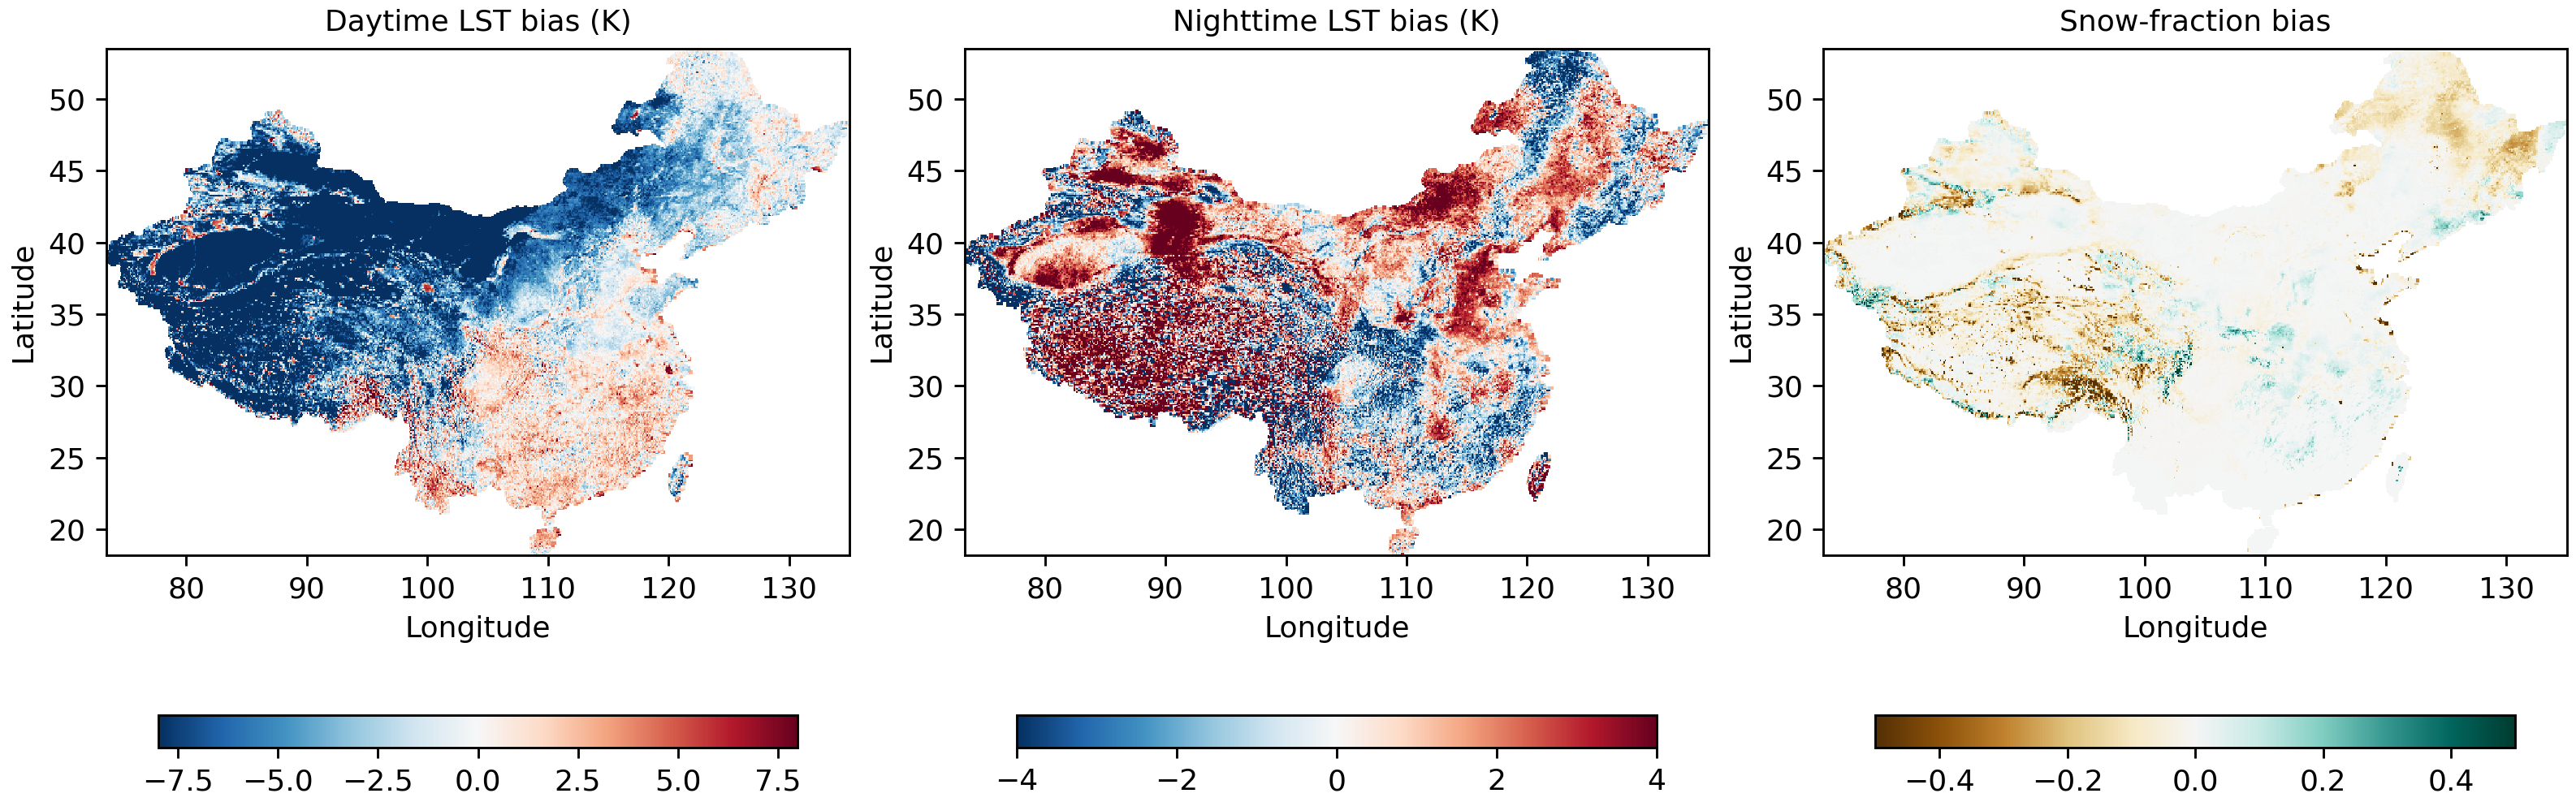
\includegraphics[width=\linewidth]{figures/modis_validation_1y_2018/modis_validation_maps.png}
\caption{Annual mean SURF-minus-MODIS differences from the spun-up
integration on the original CMFD
longitude--latitude locations. LST maps use the strict QC mask; snow uses
spatial QA 0--1 and at least 50\,\% clear coverage. Display limits are fixed
at $\pm8$~K for daytime and $\pm4$~K for nighttime LST, and $\pm0.5$ for snow
fraction; the nighttime range is half the daytime range, in proportion to the
smaller bulk spread of the nighttime bias (interquartile range $-1.3$ to
$+2.2$~K versus $-8.3$ to $+0.1$~K daytime). Untruncated aggregate statistics
are reported in Table~\ref{tab:modis-validation}.}
\label{fig:modis-maps}
\end{figure}

\begin{figure}[t]
\centering
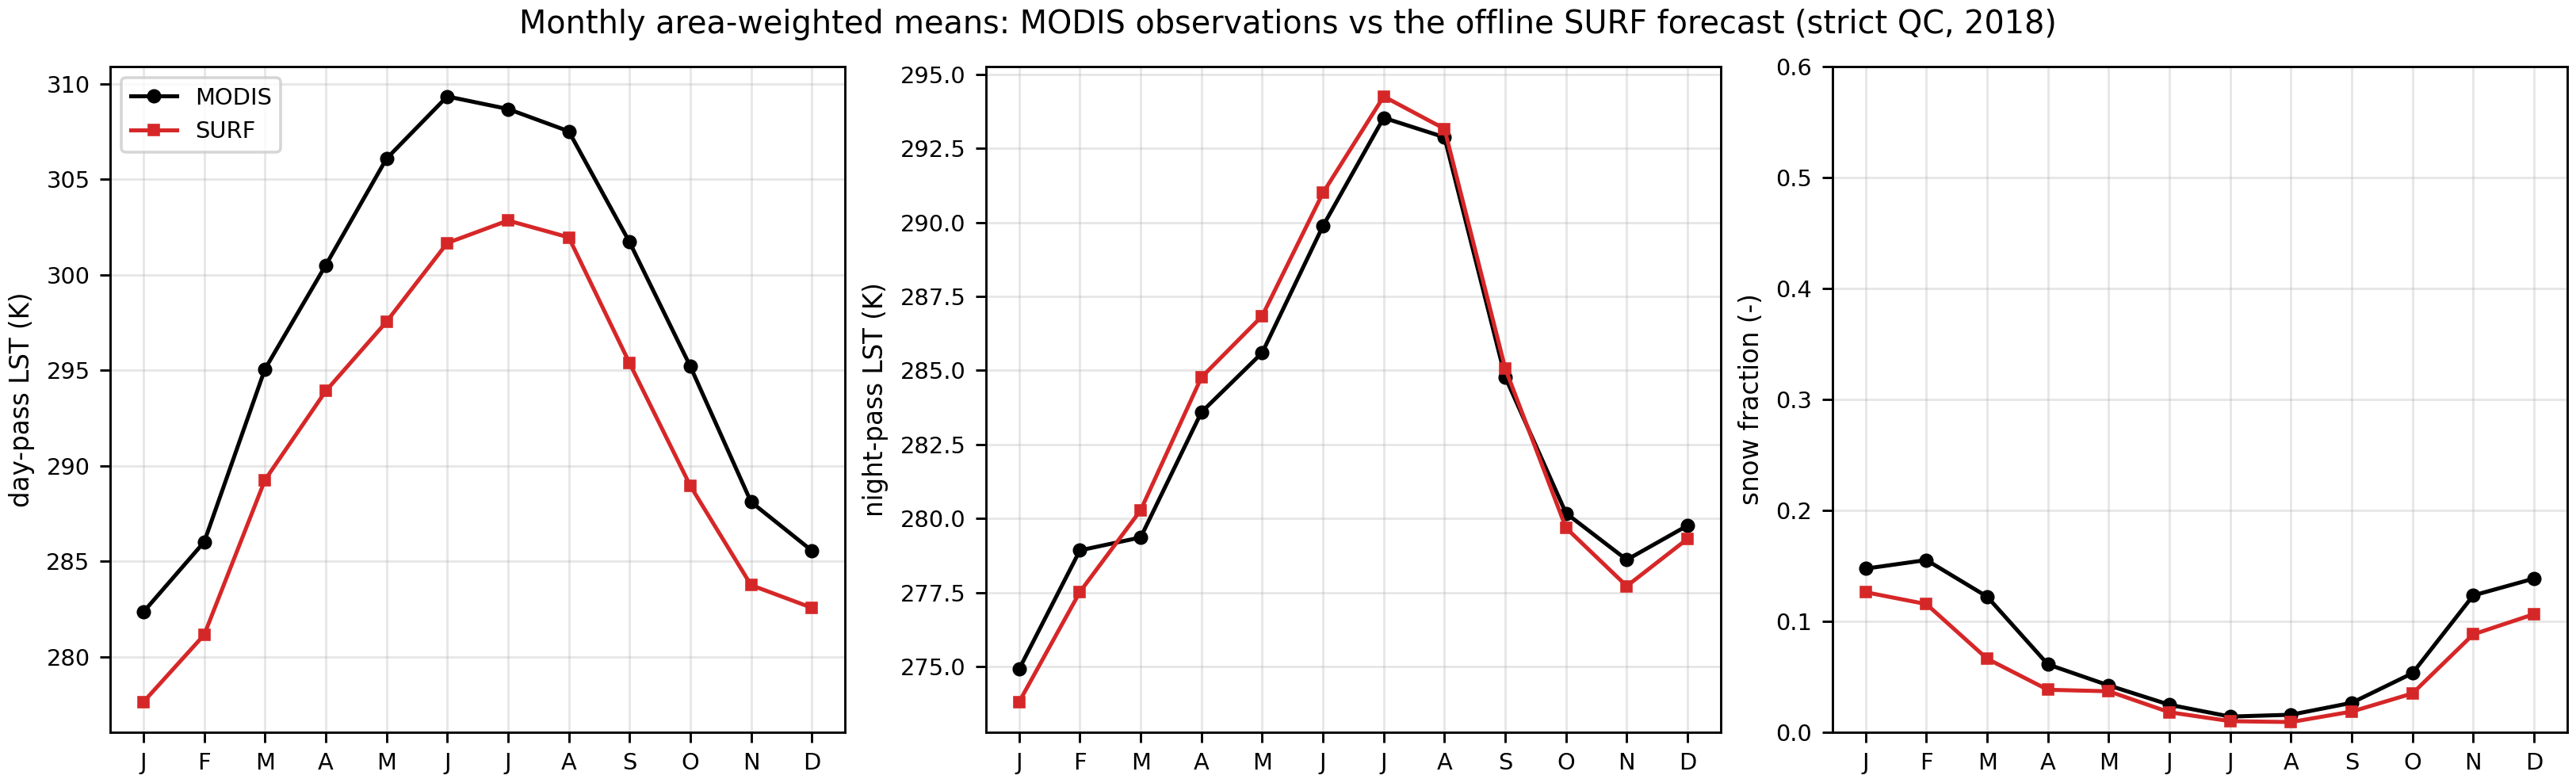
\includegraphics[width=\linewidth]{figures/modis_seasonal_cycle.png}
\caption{Monthly, area-weighted means of the MODIS observations (black) and
the offline SURF forecast (red): day-pass LST, night-pass LST, and snow
fraction (2018, spun-up initial state of
Sect.~\ref{sec:modis-evaluation}; strict QC for LST, snow QA for
snow, applied to both curves). The forecast follows the observed night-pass
cycle to within 1.4~K, under-amplifies the warm-season day-pass maximum
(forecast peak 6.5~K below observed), and reproduces the phase of the
snow cycle at a lower fraction (peak 0.11 against 0.16).}
\label{fig:modis-seasonal}
\end{figure}

\subsection{Attribution of the daytime cold bias}
\label{sec:bias-attribution}

Two checks localize the error before anything is corrected. First, global
multiplicative parameter scales contribute only a limited correction: a
gradient-based calibration of eight such scales (the vegetation
leaf-area-index, stomatal-resistance, and roughness-length tables split by
vegetation class, plus soil thermal-conductivity and dry-soil heat-capacity
scales), trained on ten autumn--winter windows and evaluated on ten
held-out spring--summer windows, removes only about $0.5$~K of the
$5.5$--$8.3$~K windowed daytime offset (7--10\,\%). This is a statement
about these eight global scales and about land surface temperature alone:
it does not exclude a larger role for other parameters (hydrological,
albedo, snow) or for other state variables. In particular, the tested
control space contains no spatially heterogeneous static fields, such as
soil texture and hydraulic properties or vegetation and albedo maps, and
the ten-day anchored windows deliberately suppress the slow soil-water
memory by restoring archived initial states. Such factors carry real
uncertainty and may contribute materially to the daytime bias; the $0.5$~K
figure is therefore a bound on this specific control space, not a general
verdict on parameter optimization, and an observing-system
simulation with the identical operator, overpass times, and optimizer
recovers imposed truth parameters to within 0.3--1.1\,\%, so the limited
correction is not an inversion failure (Appendix~\ref{app:modis-calibration}).
Second, the dominant daytime error is associated with the
offline atmosphere--surface exchange rather than with these parameter
scales: when additive air-temperature offsets and multiplicative wind and
shortwave scales are optimized instead of model parameters, the
calibration-window day bias is largely removed, and the optimal profile,
afternoon $+4.8$~K, evening $-3.1$~K, states
what is missing: the offline exchange delivers about $8.1$~K peak-to-peak
less near-surface diurnal amplitude than the observed surface demands, or an
equivalent radiative gain. The same corrections retain most of their
effect in the held-out season under the anchored-day evaluation, so the
profile is seasonally robust; it remains a diagnosis rather than a
correction, as a ten-control additive adjustment of one year's forcing has
no process form
(Appendix~\ref{app:modis-calibration}).

The attribution experiment is enabled by the differentiable formulation.
With the role of the model parameters bounded, the residual bias
is interrogated from the forcing side: a pseudo-forcing correction,
additive air-temperature offsets in the eight local-time 3-hour bins plus
multiplicative scales on wind and shortwave, ten controls in all, is
optimized against the same MODIS loss. A finite-difference probe identifies
the day-overpass bin and the shortwave scale as the dominant levers, and
gradients of the loss with respect to all ten controls are obtained from a
single reverse pass through the unrolled trajectory, so the full diurnal
profile is adjusted jointly. Trained on the ten autumn--winter days, the
optimization removes most of the calibration-window daytime bias ($-5.48$ to
$-1.44$~K; RMSE $7.45$ to $5.11$~K) and converges to a definite profile,
afternoon $+4.8$~K, evening $-3.1$~K
(Fig.~\ref{fig:modis-attribution}). The profile constitutes the functional
form of the missing process: the offline exchange under-delivers
near-surface diurnal amplitude in the afternoon and over-delivers it in the
evening, a deficit of about $8.1$~K peak-to-peak that no single parameter
scale can represent. The same corrections keep most of their effect in the
held-out spring--summer evaluation (day bias $-8.28$ to $-3.97$~K), so the
diagnosed shape is seasonally robust; the profile is interpreted as a
diagnosis of the missing process rather than as a correction, and it
provides the design
basis for the closure of the next subsection.

What this experiment does and does not establish deserves to be stated
explicitly. The optimized profile is a projection of the model--observation
residual onto a deliberately chosen, ten-dimensional forcing-side control
space, and it is compensatory by construction: it shows how the forcing
would have to change for the present model to reproduce the observed
surface, not how the forcing actually errs. In particular, the profile is
not evidence of a several-kelvin defect in the CMFD air temperature: a
literal forcing-error reading would require a station-fused product, whose
daily-scale temperatures are well validated \citep{He2020CMFD}, to carry a
sign-changing sub-daily bias of about $5$~K amplitude within the daytime
hours, which is implausible. Whether CMFD carries any such sub-daily error
is immaterial to the argument and is left to dedicated validation against
station observations. Whether the diagnosed deficit originates in the
forcing data, in the one-way offline coupling, which permits no two-way
adjustment between the land surface and the near-surface atmosphere, or in
the land-side exchange formulation cannot be separated within this
framework, and none of the conclusions below depends on resolving that
question. What the probe does establish is threefold: the channel through
which the daytime error is transmitted most strongly (the exchange air
temperature; Appendix~\ref{sec:forcing-sensitivity}); the functional form
the correction must have (a sign change within the daytime hours, which no
time-constant parameter in any control space can express); and, through
the wind scale settling below unity at $0.72$, internal evidence that the
offline configuration couples the surface too strongly to the imposed
atmosphere.

Two features of the attribution explain why the closure of the next
subsection acts on the exchange air temperature rather than on the other
forcings. First, the leverage is not shared evenly: the finite-difference
probe identifies the daytime overpass air temperature and the shortwave as
the dominant levers, while the wind scale is far weaker. Second, the wind
and shortwave corrections are not separable from the air-temperature one:
over the optimization the wind scale settles at $0.72$ while the shortwave
scale stays at its initial value of $1.0$, so the radiative correction is
redundant once the air-temperature profile is free to move. The
air-temperature profile, by contrast,
yields a unique and physically interpretable shape, the missing
near-surface diurnal amplitude, and the radiative gain it implicitly
requires is energetically equivalent to a shortwave correction. Acting on
the exchange air temperature therefore captures the dominant, unambiguous
part of the diagnosed deficit, while the wind part is
largely represented by the same amplitude correction. An independent
single-channel sensitivity check confirms this ordering: the exchange air
temperature drives daytime LST an order of magnitude more strongly than
every other forcing channel (five times the next strongest, thirty times
the shortwave; Appendix~\ref{sec:forcing-sensitivity}), so it is the
channel through which the daytime deficit is transmitted most strongly.

\begin{figure}[t]
\centering
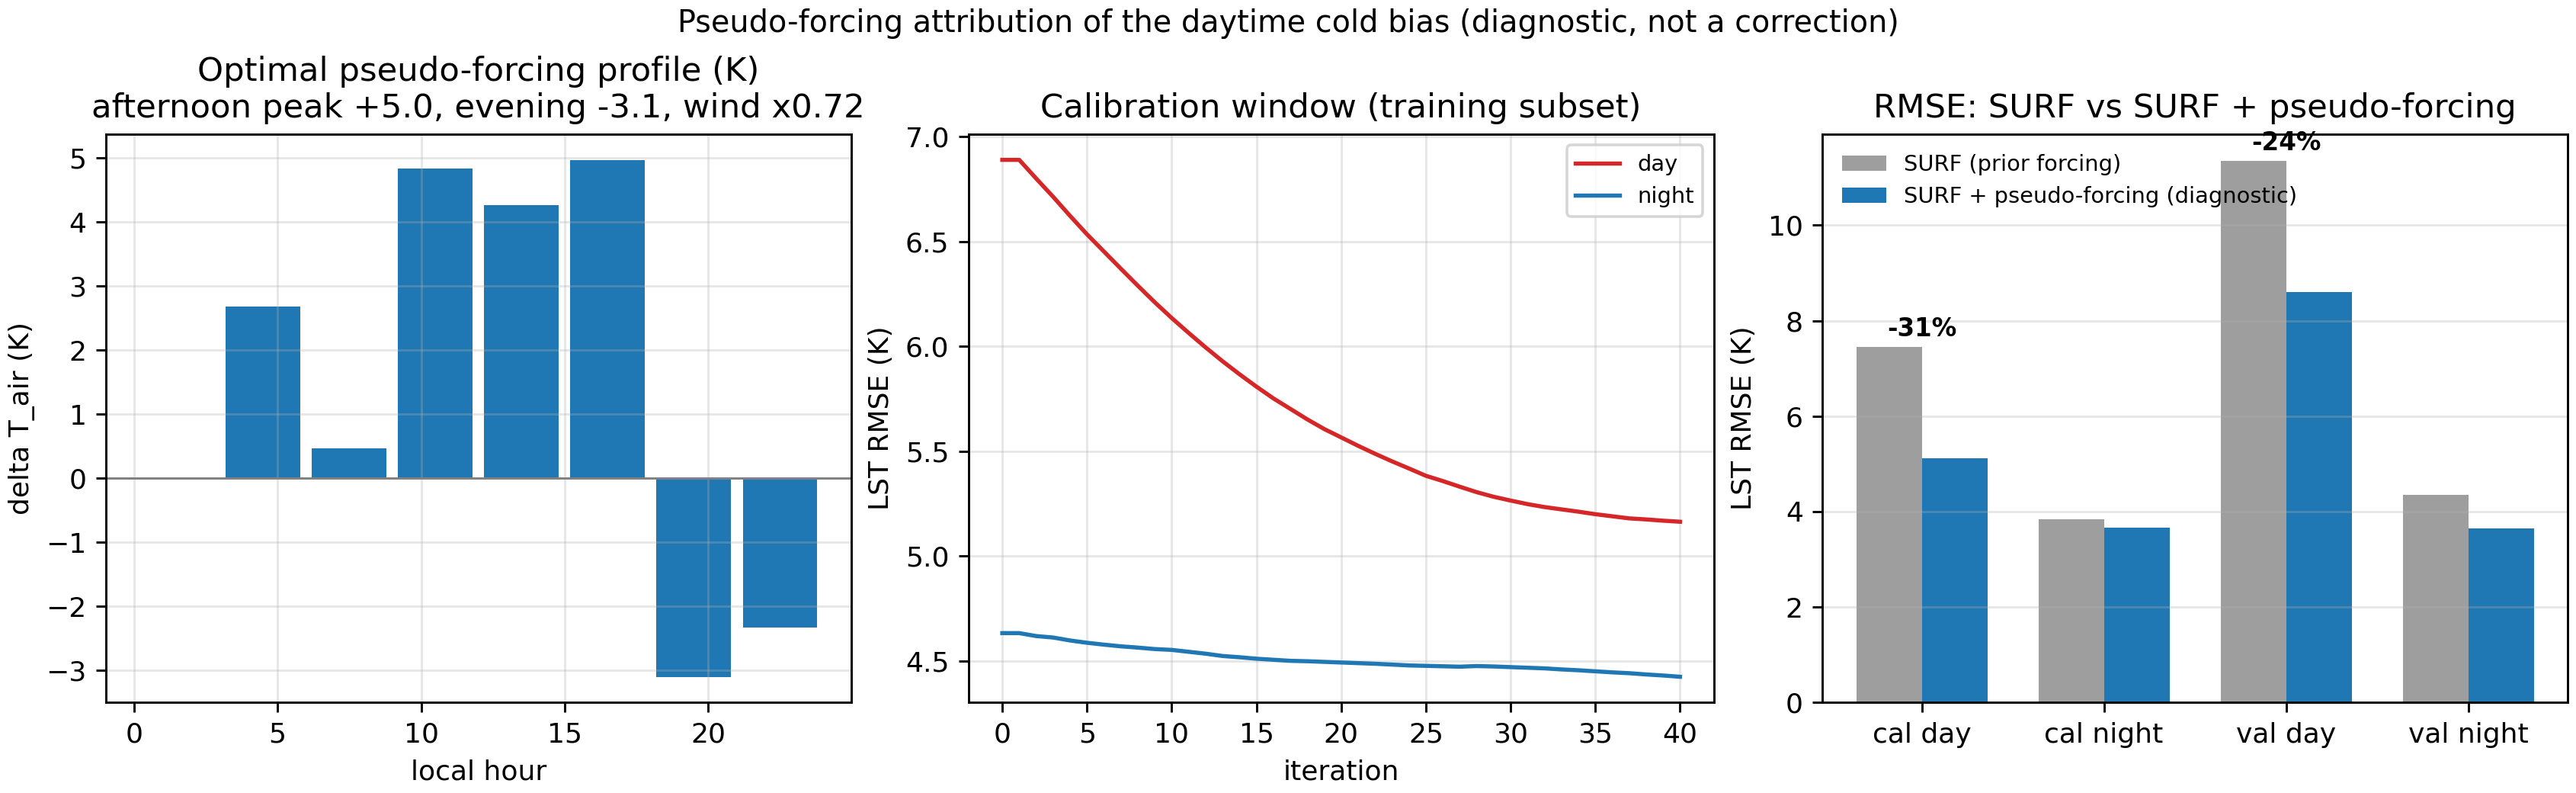
\includegraphics[width=\linewidth]{figures/modis_structural_attribution.png}
\caption{Pseudo-forcing attribution of the daytime cold bias (diagnostic,
not a parameterization). Left: the optimized additive air-temperature
profile by local 3-hour bin (bars; afternoon peak $+5.0$~K, evening
$-3.1$~K, wind $\times0.72$, shortwave unmoved); the profile expresses, in
forcing units, the correction the observations require of the near-surface
diurnal amplitude of the offline exchange (about $8.1$~K peak-to-peak); it
is not an estimate of forcing-data error. Centre: day and
night LST RMSE over the calibration-window training subset during the
ten-control optimization. Right: full-domain LST
RMSE with prior forcing versus with the pseudo-forcing applied
(SURF vs SURF~+~pseudo-forcing), in the calibration and held-out windows;
the corrections retain most
of their effect in the held-out season under the anchored-day protocol
(day RMSE $-24$\,\%), and the profile is used only as a diagnosis of the
missing near-surface diurnal amplitude, not as a model configuration.}
\label{fig:modis-attribution}
\end{figure}

\subsection{Observation-constrained design of a finite-capacity surface-layer closure}
\label{sec:structural-slab}

We therefore complement parameter calibration with a process-level
representation of the unresolved near-surface coupling. Because the probe
cannot separate forcing error from missing coupling physics, the closure is
designed as a parameterization of the missing process, not as a correction
of the forcing data.

\begin{figure}[t]
\centering
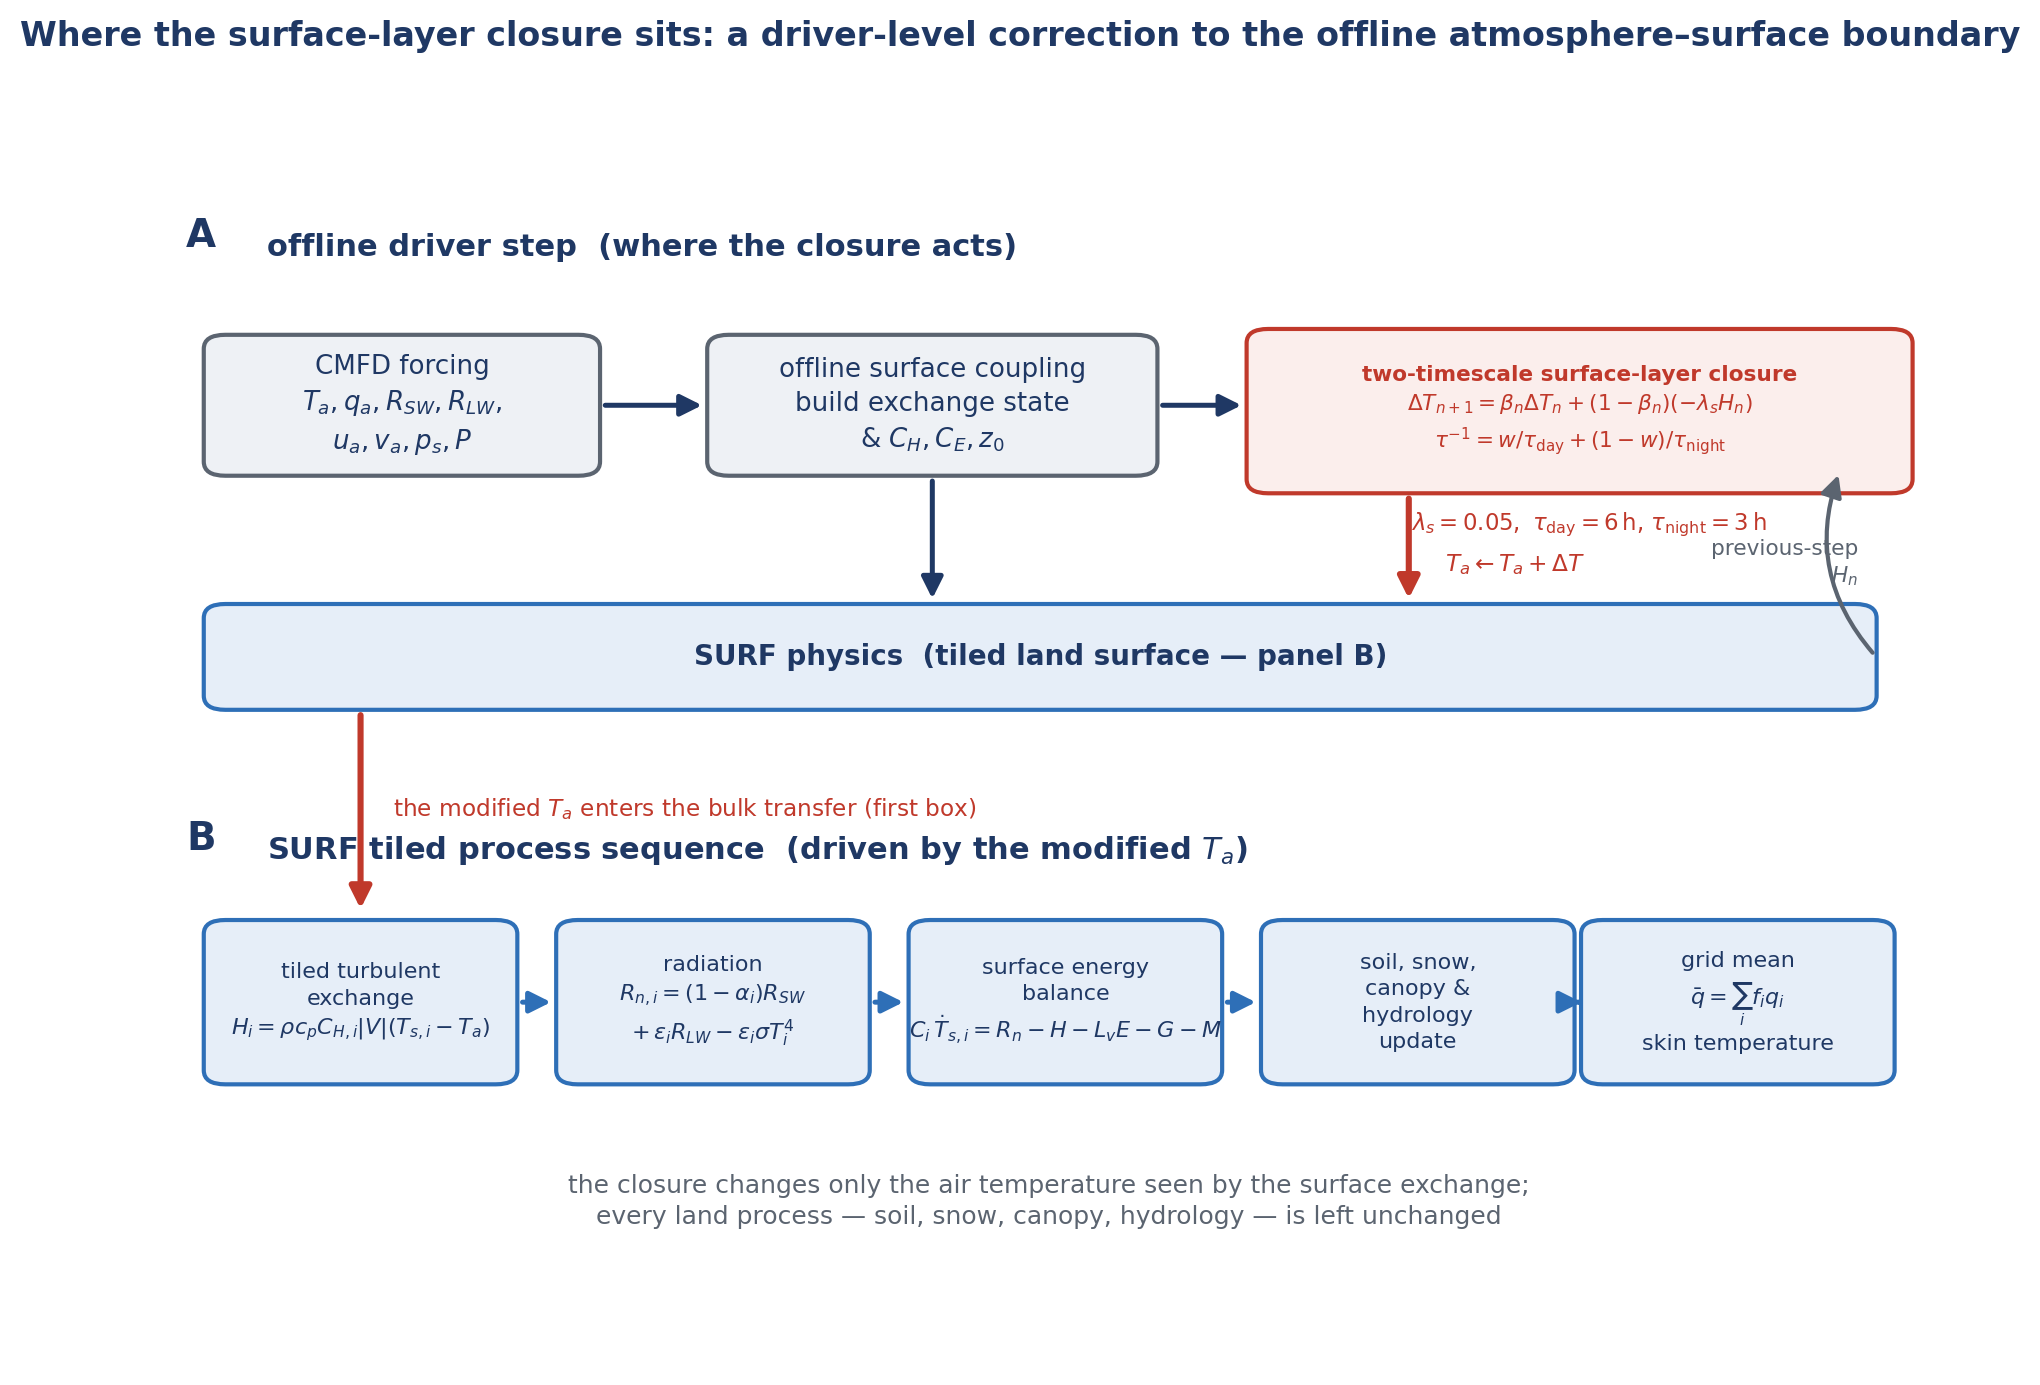
\includegraphics[width=\linewidth]{figures/modis_closure_schematic.png}
\caption{Where the surface-layer closure sits in the offline model. Panel A:
the driver step. The closure modifies only the exchange air temperature $T_a$
after the offline surface coupling is built and before the SURF physics is
called, a driver-level correction to the atmosphere--surface boundary, not
a new land process. Panel B: the tiled SURF process sequence that the modified
$T_a$ then drives; every land process (soil, snow, canopy, hydrology) is left
unchanged.}
\label{fig:closure-schematic}
\end{figure}

The closure interprets the reanalysis air temperature as a forcing anchored
above a finite-capacity surface layer, whose anomaly $\Delta T$ tracks the
quasi-steady exchange offset $-\lambda_s H$ under the surface sensible heat
flux $H$ (downward positive, Fig.~\ref{fig:closure-schematic}):
\begin{equation}
\frac{\mathrm{d}\Delta T}{\mathrm{d}t} = \frac{-\lambda_s H - \Delta T}{\tau(t)},
\qquad
\tau(t)^{-1} = \frac{w}{\tau_{\mathrm{day}}} + \frac{1 - w}{\tau_{\mathrm{night}}},
\qquad
w = \frac{S}{S + 50~\mathrm{W\,m^{-2}}},
\label{eq:slab}
\end{equation}
where $S$ is the surface downward shortwave of the step, so the day--night
transition follows sunrise, sunset, and cloudiness rather than a clock.
Discretized explicitly per physics step,
$\Delta T_{n+1} = \beta_n \Delta T_n + (1-\beta_n)(-\lambda_s H_n)$ with
$\beta_n = \exp(-\Delta t/\tau_n)$, and applied to the exchange air
temperature only, the closure has three constants: the coupling coefficient
$\lambda_s$ sets the amplitude of the correction, and the two relaxation
times set how fast the surface layer tracks it (an effective depth $h =
\tau/(\rho c_p \lambda_s)$). Two properties matter. First, the relaxation
term is not optional: the undamped quasi-steady form $\Delta T = -\lambda_s
H$ is a positive feedback under nocturnal stable stratification, and the
first version of this experiment demonstrated the consequence numerically:
the
integration produces non-finite states at $\lambda_s \approx 0.03$~K\,(W\,m$^{-2}$)$^{-1}$.
Second, $\lambda_s = 0$ reproduces the baseline bitwise, so the closure
changes nothing until it is calibrated.

The calibration protocol mirrors Appendix~\ref{app:modis-calibration} and
is stated here in full. The training windows are ten autumn--winter days of
2018 (days of year 271, 281, $\dots$, 361) and the held-out windows ten
spring--summer days (days of year 91, 101, $\dots$, 181); no
spring--summer state ever enters a training loss. For every window the land
state is restored from the daily archive of the autonomous, unclosed 2018
integration of Sect.~\ref{sec:modis-evaluation} at the preceding day
boundary; the closure is switched on during a one-day (48-step) build-up
integrated without gradients, so that its memory state equilibrates before
the scored window, and the following 48-step forecast day carries
gradients. The forcing throughout is the same CMFD 2018 three-hourly
field set, interpolated to the 1800~s physics step, as the autonomous run
(Sect.~\ref{sec:fortran-torch-equivalence}). The loss is the
$\cos\phi$-weighted day-plus-night mean-squared strict-QC LST residual over
every fifth CMFD column (19{,}542 of 97{,}709). Within the recurrence, the
flux entering the quasi-steady target is treated as constant per step, so
gradients propagate through the anomaly recursion and its direct effect on
the exchange air temperature, not through the flux feedback. Stage one
trains the coupling coefficient itself (Adam, learning rate 0.004 from an
initial value of $10^{-3}$~K\,(W\,m$^{-2}$)$^{-1}$, 40 iterations); stage
two optimizes the two timescales jointly by Adam on their logarithms
(learning rate 0.05, 40 iterations). In both stages an
iteration whose gradients are not finite is rejected and leaves the
parameters at their last stable value. The
three constants are calibrated
in two stages on the same ten autumn--winter days. In the first stage the
two timescales are tied through a fixed effective depth ($h_s = 600$~m,
i.e.\ $\tau_s = \lambda_s \rho c_p h_s$) and the single free parameter
$\lambda_s$ settles at its upper bound of
$0.05$~K\,(W\,m$^{-2}$)$^{-1}$ ($\tau_s \approx 10$~h): the data ask for the
strongest admissible coupling, and the bound-seeking behaviour locates the
remaining error in how quickly the layer tracks that coupling. In the
second stage $\lambda_s = 0.05$ is held fixed and the two relaxation times
are trained by the same gradient machinery, the identical Adam
calibration, loss, and strided column subset, with the times
parameterized in log space and initially bounded to $[2,12]$~h. Started
from the tied value of $10.1$~h for both, the optimizer separates the
timescales within about 30 accepted steps and becomes stationary at
$\tau_{\mathrm{day}} = 2.47$~h and $\tau_{\mathrm{night}} = 2.36$~h (training
loss 481 to 401 on the calibration subset); the trailing iterations are
then rejected by the non-finite-gradient guard, because the optimizer has
walked
to the edge of its own integrable range. That endpoint is unusable.
Verified step by step in state space rather than at observation times, the
held-out day-131 forecast diverges in two clusters of Tibetan-Plateau
columns ($30$--$31^\circ$N, $84$--$86^\circ$E and $37$--$38^\circ$N,
$87$--$88^\circ$E): there the grid-mean sensible heat
flux sustains an intrinsic two-step ($\sim$1~h) limit cycle even at
vanishing anomaly, and near the morning transition its sensitivity to the
exchange-air anomaly is large enough
that the closure's quasi-steady target $-\lambda_s H$ reinforces the
oscillation instead of damping it; the anomaly passes $10^{3}$~K within a
dozen steps of the dawn transition, and the first non-finite state appears
at forecast step 56 (Appendix~\ref{app:modis-calibration}).
Observation-space verification cannot see this: the strict MODIS quality
control removes the divergent columns from the sampled statistics, whose
window aggregates stay clean. The acceptance test for a learned closure
must therefore be state-space verification, applied here to the full sweep
grid over all 20 anchored evaluation days. The verified set is a resonance
structure rather than a rectangle: $\tau_{\mathrm{night}} = 2$~h
exceeds $10^{3}$~K on at least one anchored day at
$\tau_{\mathrm{day}} \in \{5, 8, 10\}$~h and stays finite but elevated at
$\tau_{\mathrm{day}} = 6$~h (worst transient 150~K), $\tau_{\mathrm{day}} =
5$~h diverges on day~121 at every $\tau_{\mathrm{night}}$ except 3~h, and
($\tau_{\mathrm{day}} = 6$~h, $\tau_{\mathrm{night}} = 5$~h) diverges on
day~121, whereas ($\tau_{\mathrm{day}} = 6$~h, $\tau_{\mathrm{night}} \in
\{3, 4\}$~h) and $\tau_{\mathrm{day}} \in \{8, 10\}$~h at
$\tau_{\mathrm{night}} \in \{3, 4, 5\}$~h pass
all 20 days with no column beyond 141~K (worst single-column
transient 109~K for the adopted combination, decaying, against 49~K for
the tied closure). Resetting
the training bounds in light of this test and repeating the gradient
calibration from the same tied start, the optimizer again presses toward
the fastest admissible tracking and settles at the verified corner,
$\tau_{\mathrm{day}} = 6$~h and $\tau_{\mathrm{night}} = 3$~h (effective
depths $\approx$360 and 180~m; training loss 433, an 8\,\% premium over
the divergent optimum that is the price of integrability). The calibrated
configuration is hereafter referred to as SURF-Opt; the uncalibrated model
remains SURF.

Table~\ref{tab:structural-closure} gives the full-domain verification of
SURF-Opt against the uncalibrated SURF. The two-timescale closure removes
67\,\% of the daytime bias in the calibration window ($-5.48$ to $-1.83$~K;
RMSE $7.45$ to $4.82$~K) and 84\,\% in the held-out spring--summer window
($-8.28$ to $-1.35$~K; RMSE $11.34$ to $7.17$~K), seven to thirteen times
the bias removal of the eight table scales of
Appendix~\ref{app:modis-calibration}. Unlike the pseudo-forcing profile,
which is an additive adjustment fitted to one year's forcing, the closure is
a process formulation: it is defined by three physical constants, carries no
per-year information, and its improvement is as large in the window
it never saw. The night passes quantify the trade-off. The
calibration-window night pass slightly improves ($-0.43$ to $-0.31$~K;
RMSE $3.83$ to $3.66$~K); the held-out night bias warms from $+1.07$ to
$+2.08$~K at essentially unchanged RMSE ($4.35$ to $4.48$~K): the daytime
heat no longer lost to the atmosphere is stored in the soil and returned
after sunset. What remains of the daytime bias is a modest cold offset
($-1.4$~K) in the held-out window; the warm nights and the shortwave
factor of the attribution experiment point at the same next structural
target, a radiative or albedo deficit that a surface-layer closure
cannot supply. Two caveats accompany these gains. First, like the probe
that motivated it, the closure is compensatory in character: it represents,
in three constants, whatever unresolved physics projects onto the
exchange-temperature channel, most plausibly the missing two-way coupling
between the surface and the near-surface atmosphere, an interpretation
consistent with the implied effective depths (360 and 180~m), which are of
the order of the diurnal heat capacity of the atmospheric surface layer.
Its credibility therefore rests on the held-out transfer reported here
rather than on a first-principles derivation. Second, the constants are
calibrated against MODIS LST under a single forcing (CMFD) and are tied to
this model--forcing combination; repeating the calibration under an
alternative forcing and validating the sub-daily structure of the exchange
level against station observations are the decisive next tests. Broader
parameter calibration, including heterogeneous static fields and slow
soil-state memory, remains complementary to, not superseded by, this
closure.

Figures~\ref{fig:modis-slab-maps} and \ref{fig:modis-slab-perday} resolve
the improvement spatially and day by day, and the monthly RMSE curves of
Fig.~\ref{fig:modis-slab-monthly} extend it to the full seasonal cycle. The
SURF daytime bias is strongest over the arid northwest and the Tibetan
Plateau and weakest over southern and northeastern China, and the closure
acts exactly where the bias lives: the box-mean day bias over the
northwestern deserts (75--105$^\circ$E, 35--48$^\circ$N) improves from
$-10.8$ to $-2.9$~K in the held-out window and over the Tibetan Plateau from
$-9.4$ to $-2.9$~K, while northeastern China shifts from $-3.1$ to
$+2.1$~K. Across all evaluated columns the absolute daytime bias
decreases at 70--76\,\%~of columns, and the fraction of columns biased by
more than 10~K drops from 16\,\%~to 2\,\%~(calibration) and from
37\,\%~to 10\,\%~(held-out). The one systematic cost is visible in the same
maps: southern China, nearly unbiased in SURF, warms by about $+3$~K,
the regional signature of the night-pass warming already quantified in
Table~\ref{tab:structural-closure}. The per-day panels show the reduction is
not an average artefact: on every one of the 20 evaluation days, in both
windows, the SURF-Opt day bias is warmer and the day RMSE lower than
SURF. The daily curves of
Fig.~\ref{fig:modis-slab-curves} show the outcome at daily resolution: in the
day pass, SURF-Opt tracks not only the observed seasonal cycle but the
day-to-day variability through the whole year, whereas SURF sits several
kelvin low in the warm season; the night-pass panel exposes the warm-season
night warming directly (about
$+2$~K in July). The monthly RMSE curves of Fig.~\ref{fig:modis-slab-monthly} extend
the check to the full seasonal cycle, from continuous year-long integrations:
the day-pass RMSE decreases in every month of the year (by $0.9$--$4.4$~K,
largest in May), while the night-pass cost is confined to May--August (at
most $0.6$~K, in 4 of 12 months); the cold-season night pass is unchanged
to slightly improved.

Because the closure acts only on the exchange-level air temperature and the
grid-mean sensible heat flux, physical quantities computed identically in
either implementation, it requires no differentiable infrastructure to
apply: the identical recurrence has been implemented at
the driver level of the Fortran offline model, where the compiled-in default
$\lambda_s = 0$ reproduces the unpatched driver bitwise
(Appendix~\ref{app:fortran-slab}).

\begin{table}[t]
\caption{Full-domain MODIS LST verification of SURF-Opt
against the uncalibrated spun-up SURF. ``SURF-Opt'' is the optimized
configuration of Eq.~(\ref{eq:slab}) with $\lambda_s =
0.05$~K\,(W\,m$^{-2}$)$^{-1}$ and gradient-calibrated relaxation times
($\tau_{\mathrm{day}} = 6$~h, $\tau_{\mathrm{night}} = 3$~h, on the
state-space-verified stability boundary) obtained by the two-stage
calibration on the ten autumn--winter days.
The diagnostic experiments of Appendix~\ref{app:modis-calibration} are not
model configurations and are therefore not tabulated: the eight-control
table-scale calibration removes at most 0.5~K of the daytime bias within
that tested control space, and the
ten-control pseudo-forcing attribution removes most of the calibration-window
day
bias ($-5.48$ to $-1.44$~K, RMSE $7.45$ to $5.11$~K) and retains most of
that reduction in the held-out window (day bias $-8.28$ to $-3.97$~K).}
\label{tab:structural-closure}
\centering
\small
\begin{tabular}{llrrrr}
\hline
Window & Pass & \multicolumn{2}{c}{SURF} & \multicolumn{2}{c}{SURF-Opt} \\
 & & bias (K) & RMSE (K) & bias (K) & RMSE (K) \\
\hline
Calibration (autumn--winter) & day & $-5.48$ & $7.45$ & $-1.83$ & $4.82$ \\
 & night & $-0.43$ & $3.83$ & $-0.31$ & $3.66$ \\
Held-out (spring--summer) & day & $-8.28$ & $11.34$ & $-1.35$ & $7.17$ \\
 & night & $+1.07$ & $4.35$ & $+2.08$ & $4.48$ \\
\hline
\end{tabular}
\end{table}

\begin{figure}[t]
\centering
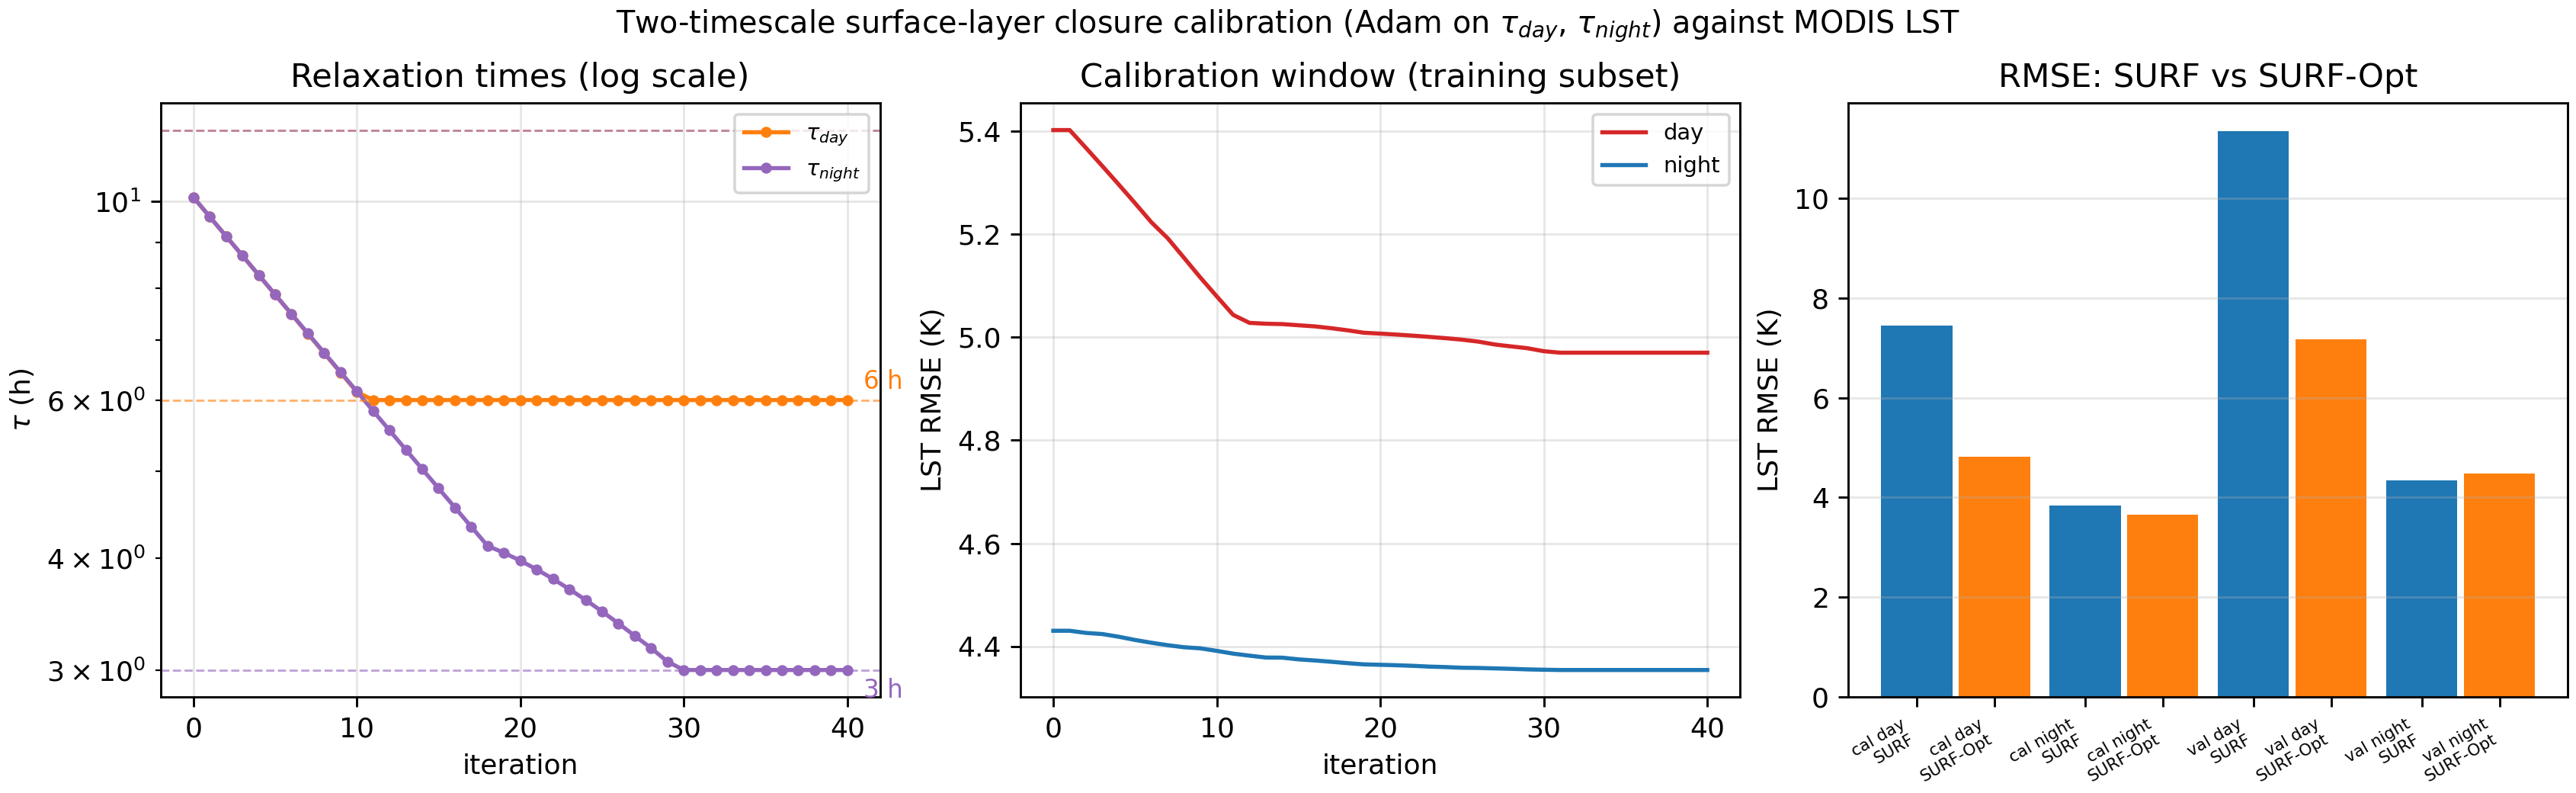
\includegraphics[width=\linewidth]{figures/modis_structural_slab.png}
\caption{Two-timescale surface-layer closure calibration
(Eq.~(\ref{eq:slab})). Left: trajectories of the two relaxation times under
Adam on $(\log\tau_{\mathrm{day}}, \log\tau_{\mathrm{night}})$, started from
the tied value of $10.1$~h and settling at the corner of the
state-space-verified set (dashed: the training bounds
$6 \le \tau_{\mathrm{day}} \le 12$~h and $3 \le \tau_{\mathrm{night}} \le
12$~h; the
unconstrained endpoint at $(2.47, 2.36)$~h lies outside it and diverges).
Centre: calibration-window day and night LST RMSE over the training
subset. Right: SURF-versus-SURF-Opt full-domain RMSE in the calibration and
held-out windows: the day-pass improvement transfers to the window never used
in training.}
\label{fig:modis-structural-slab}
\end{figure}

\begin{figure}[t]
\centering
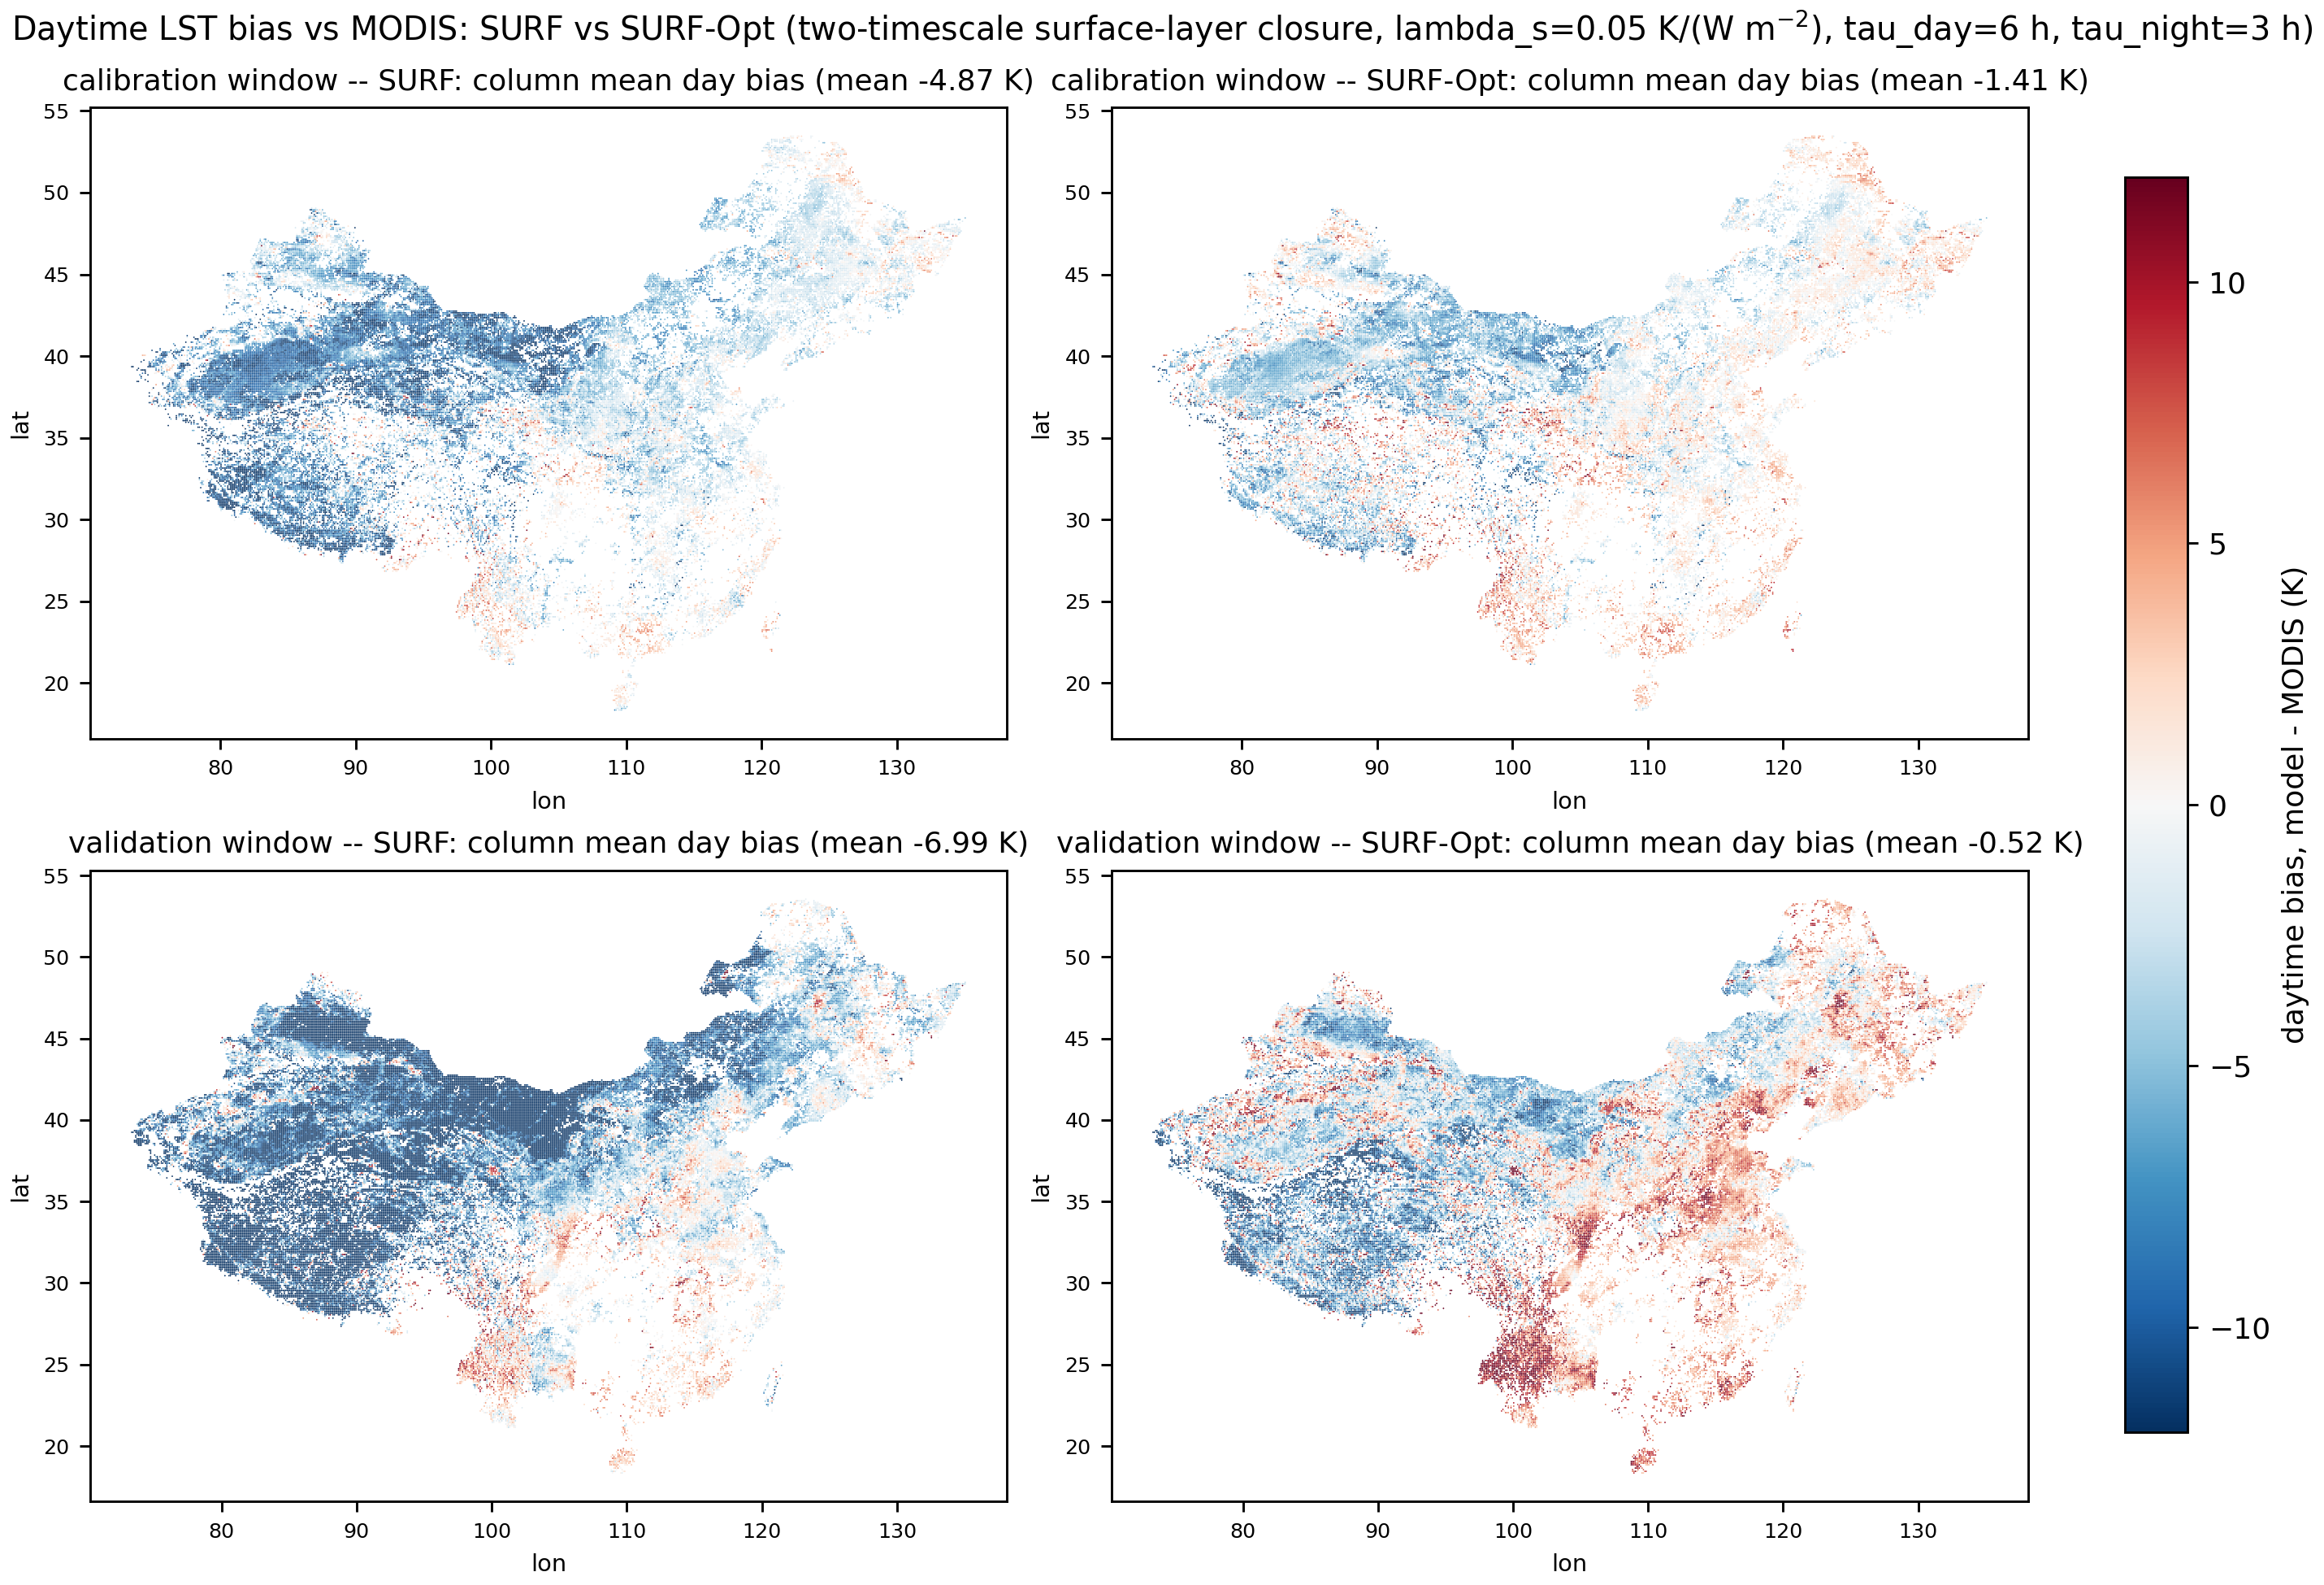
\includegraphics[width=\linewidth]{figures/modis_slab_maps.png}
\caption{Column-mean daytime LST bias against MODIS for SURF (left) and
SURF-Opt (right), in the calibration window (top row) and the held-out
spring--summer window (bottom row). Panel titles give the area-weighted
window mean; all panels share a divergent colour scale ($\pm 12$~K). The
closure acts where the bias lives: the strong cold biases over the arid
northwest and the Tibetan Plateau are largely removed, while nearly
unbiased southern China warms by about $+3$~K, the regional signature of
the night-pass warming quantified in
Table~\ref{tab:structural-closure}.}
\label{fig:modis-slab-maps}
\end{figure}

\begin{figure}[t]
\centering
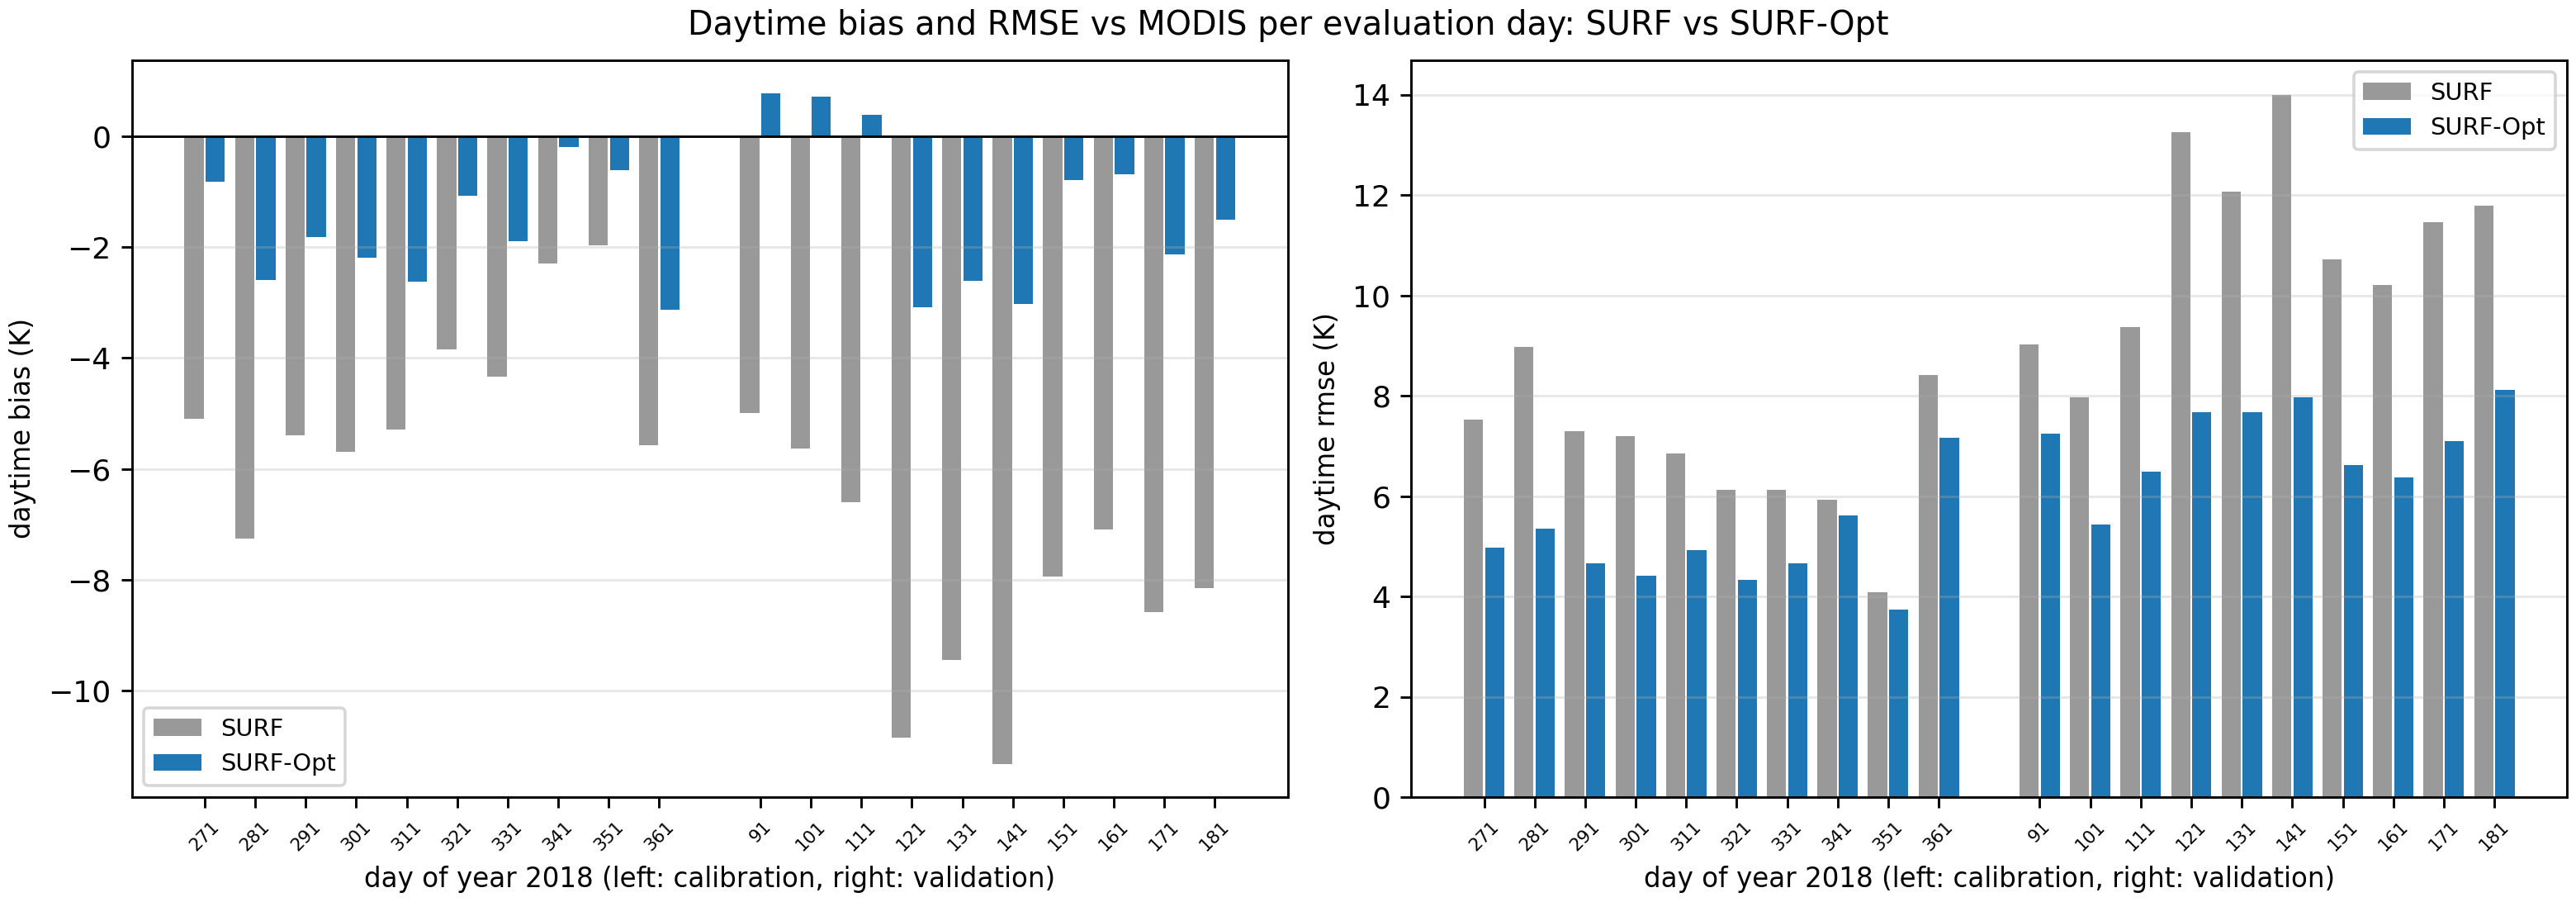
\includegraphics[width=\linewidth]{figures/modis_slab_perday.png}
\caption{Per-evaluation-day, area-weighted daytime bias (left) and RMSE
(right) against MODIS for SURF (grey) and SURF-Opt (blue),
over the ten calibration days (days of year 271--361) and the ten held-out
spring--summer days (days of year 91--181).}
\label{fig:modis-slab-perday}
\end{figure}

\begin{figure}[t]
\centering
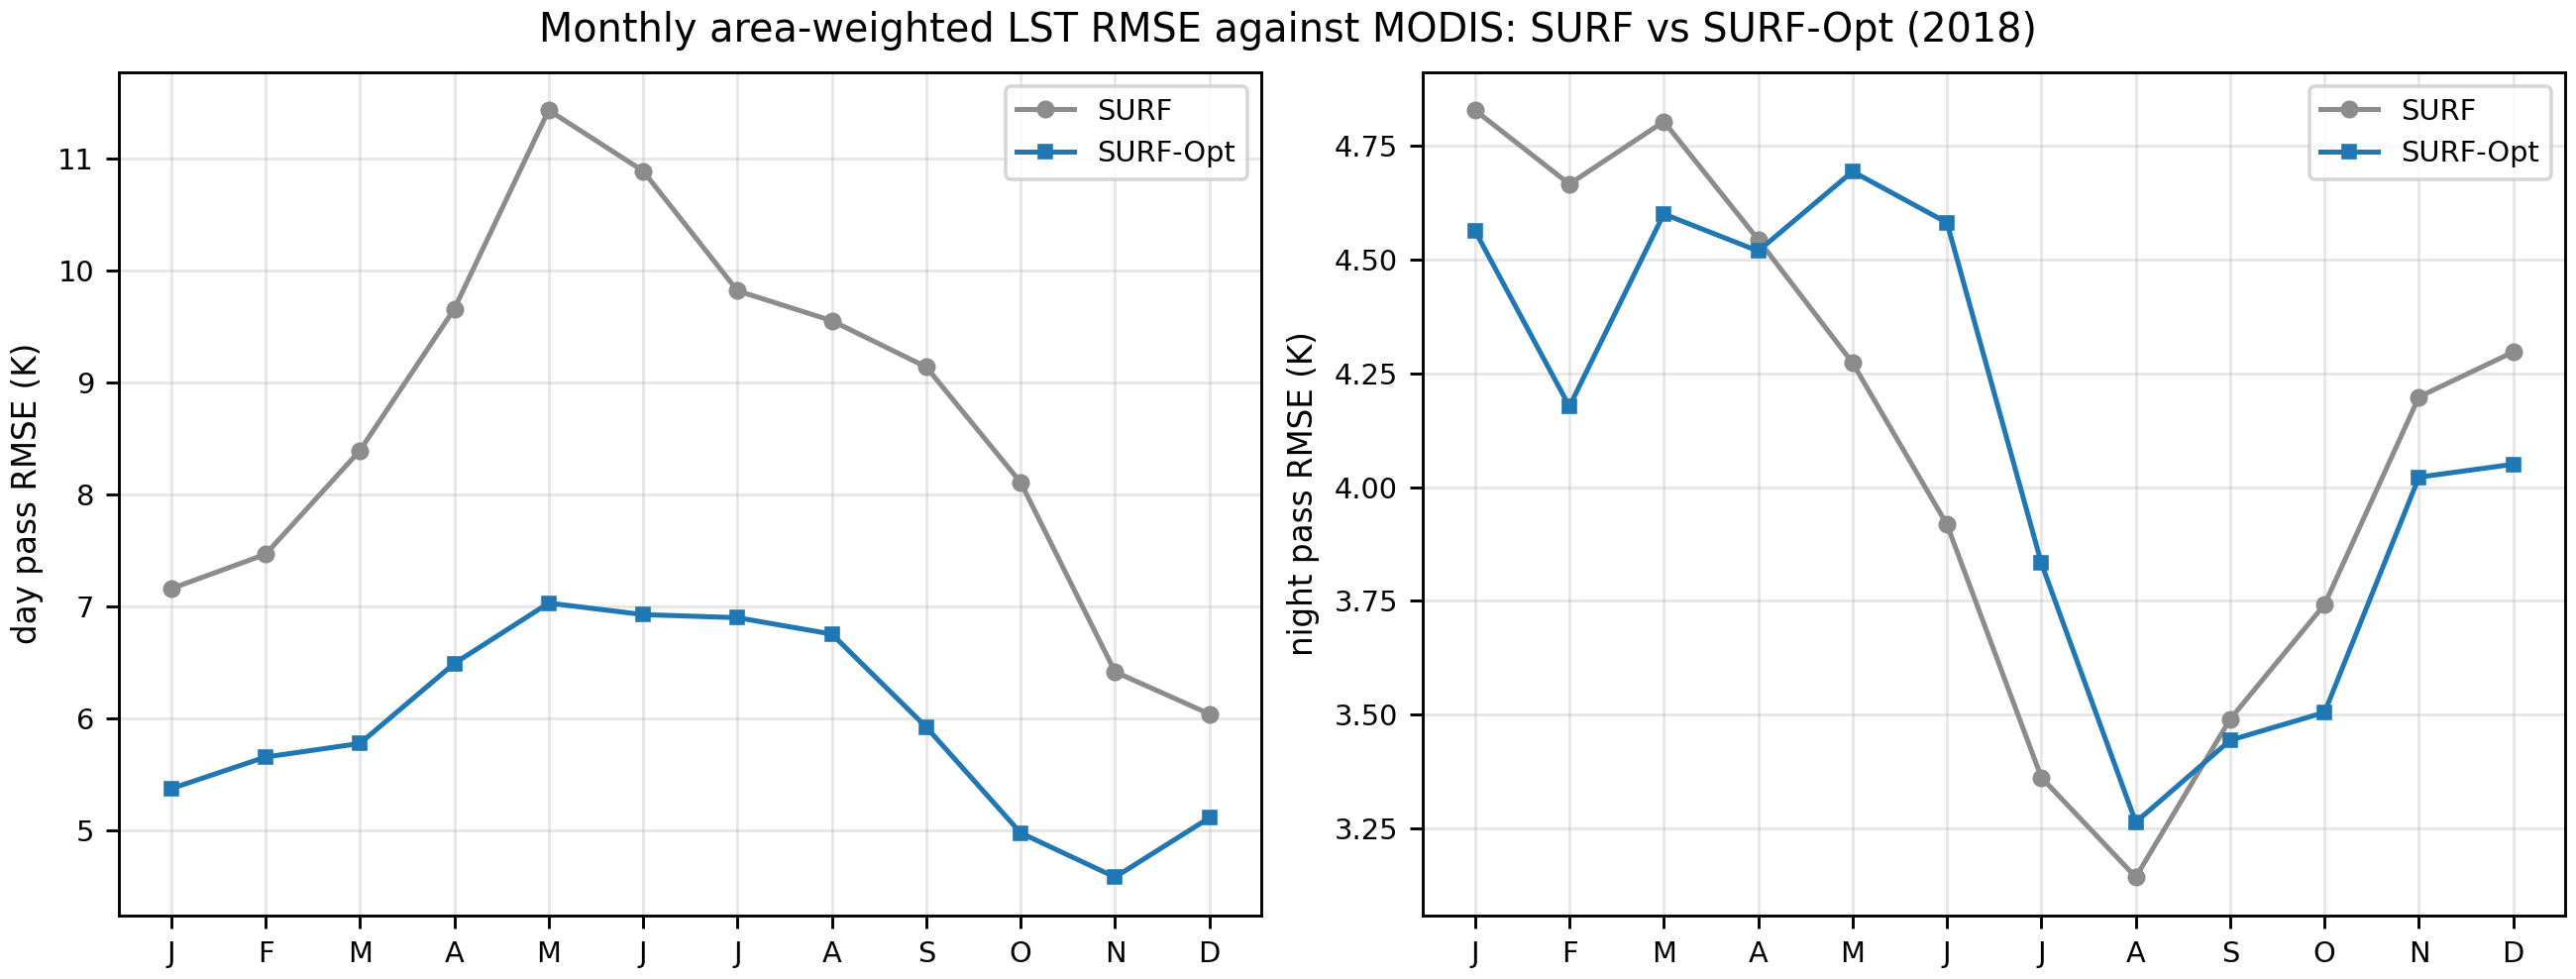
\includegraphics[width=\linewidth]{figures/modis_slab_monthly.png}
\caption{Monthly, area-weighted LST RMSE against MODIS (strict QC) for the
SURF (grey) and SURF-Opt (blue), day pass (left) and night pass
(right), from continuous full-year 2018 integrations of the torch
implementation under the observation operator of
Sect.~\ref{sec:modis-evaluation}. The day-pass RMSE is lower in every
month; the night-pass degradation is confined to March--September.}
\label{fig:modis-slab-monthly}
\end{figure}

\begin{figure}[t]
\centering
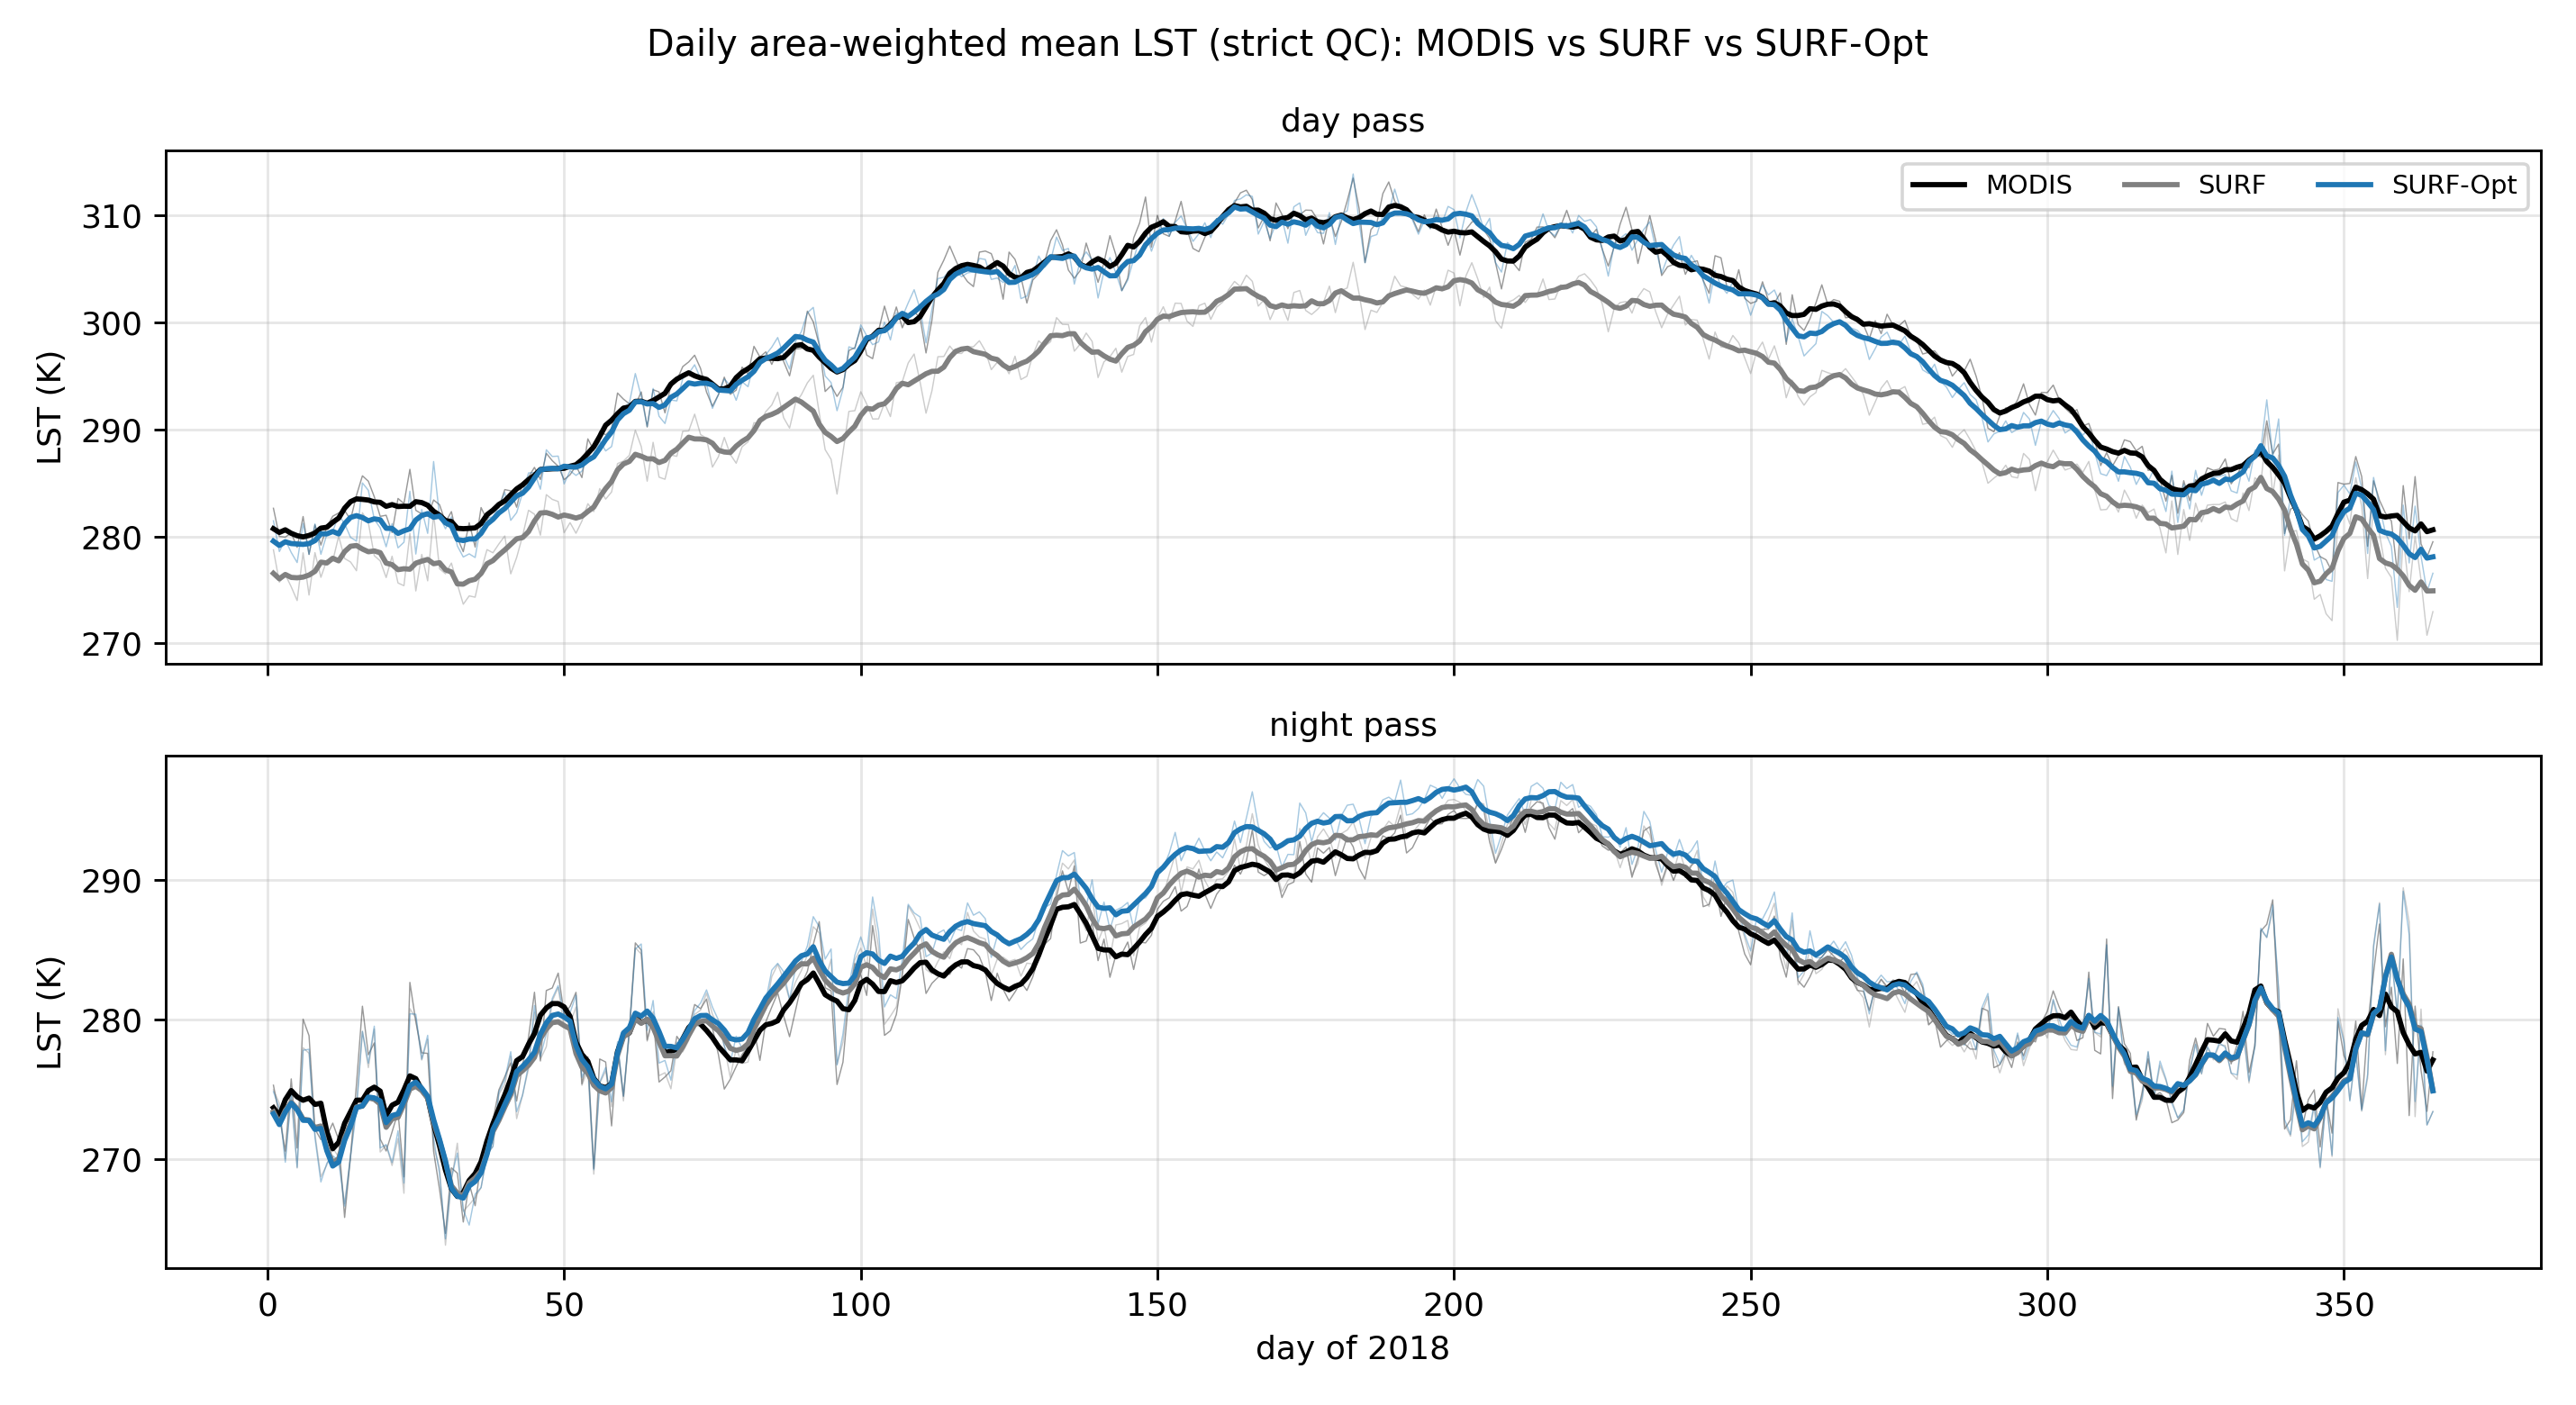
\includegraphics[width=\linewidth]{figures/modis_slab_daily_curves.png}
\caption{Daily, area-weighted mean LST from the same continuous year-long
integrations (strict QC): MODIS (black), SURF (grey), and SURF-Opt (blue),
for the day pass (top) and the night pass (bottom). Thin lines are the daily
values, thick lines a seven-day running mean. In the day pass, SURF-Opt
tracks the observed seasonal cycle and its day-to-day variability through
the whole year, whereas SURF sits several kelvin low in the warm season;
the night-pass panel exposes the warm-season night warming directly (about
$+2$~K in July). The monthly-mean view of the SURF forecast against the
same observations is given in Fig.~\ref{fig:modis-seasonal}.}
\label{fig:modis-slab-curves}
\end{figure}
